\section{Task and Evaluation}\label{sec:construction}\label{sec:benchmarks}\label{sec:setup}\label{sec:problem}\label{sec:breadth}\label{sec:models}

Admission stores $K\subseteq C$, $|K|\leq k$, from passage $x$ and ordered candidates $C=(c_1,\ldots,c_m)$ before future question $q$ and answer $a$ are known. When $q$ arrives, the frozen reader sees only $q$ and $K$. Every policy receives identical candidates and budget.

Each episode centers on a useful concept linking the passage to a future answer (Figure~\ref{fig:episode}). Test episodes follow the Decoupled construction: recover the useful concept, then combine it with general knowledge. GPT-4.1 writes a passage about a named person together with the useful concept, question and answer. The answer is excluded from passage and candidates; the question connects to the passage only through the person's name. The generator's gold utility labels mark the useful concept positive and other candidates negative; rule-based and blind alias filters check episodes (App.~\ref{app:benchmarks}).

\begin{figure*}[t]
\centering
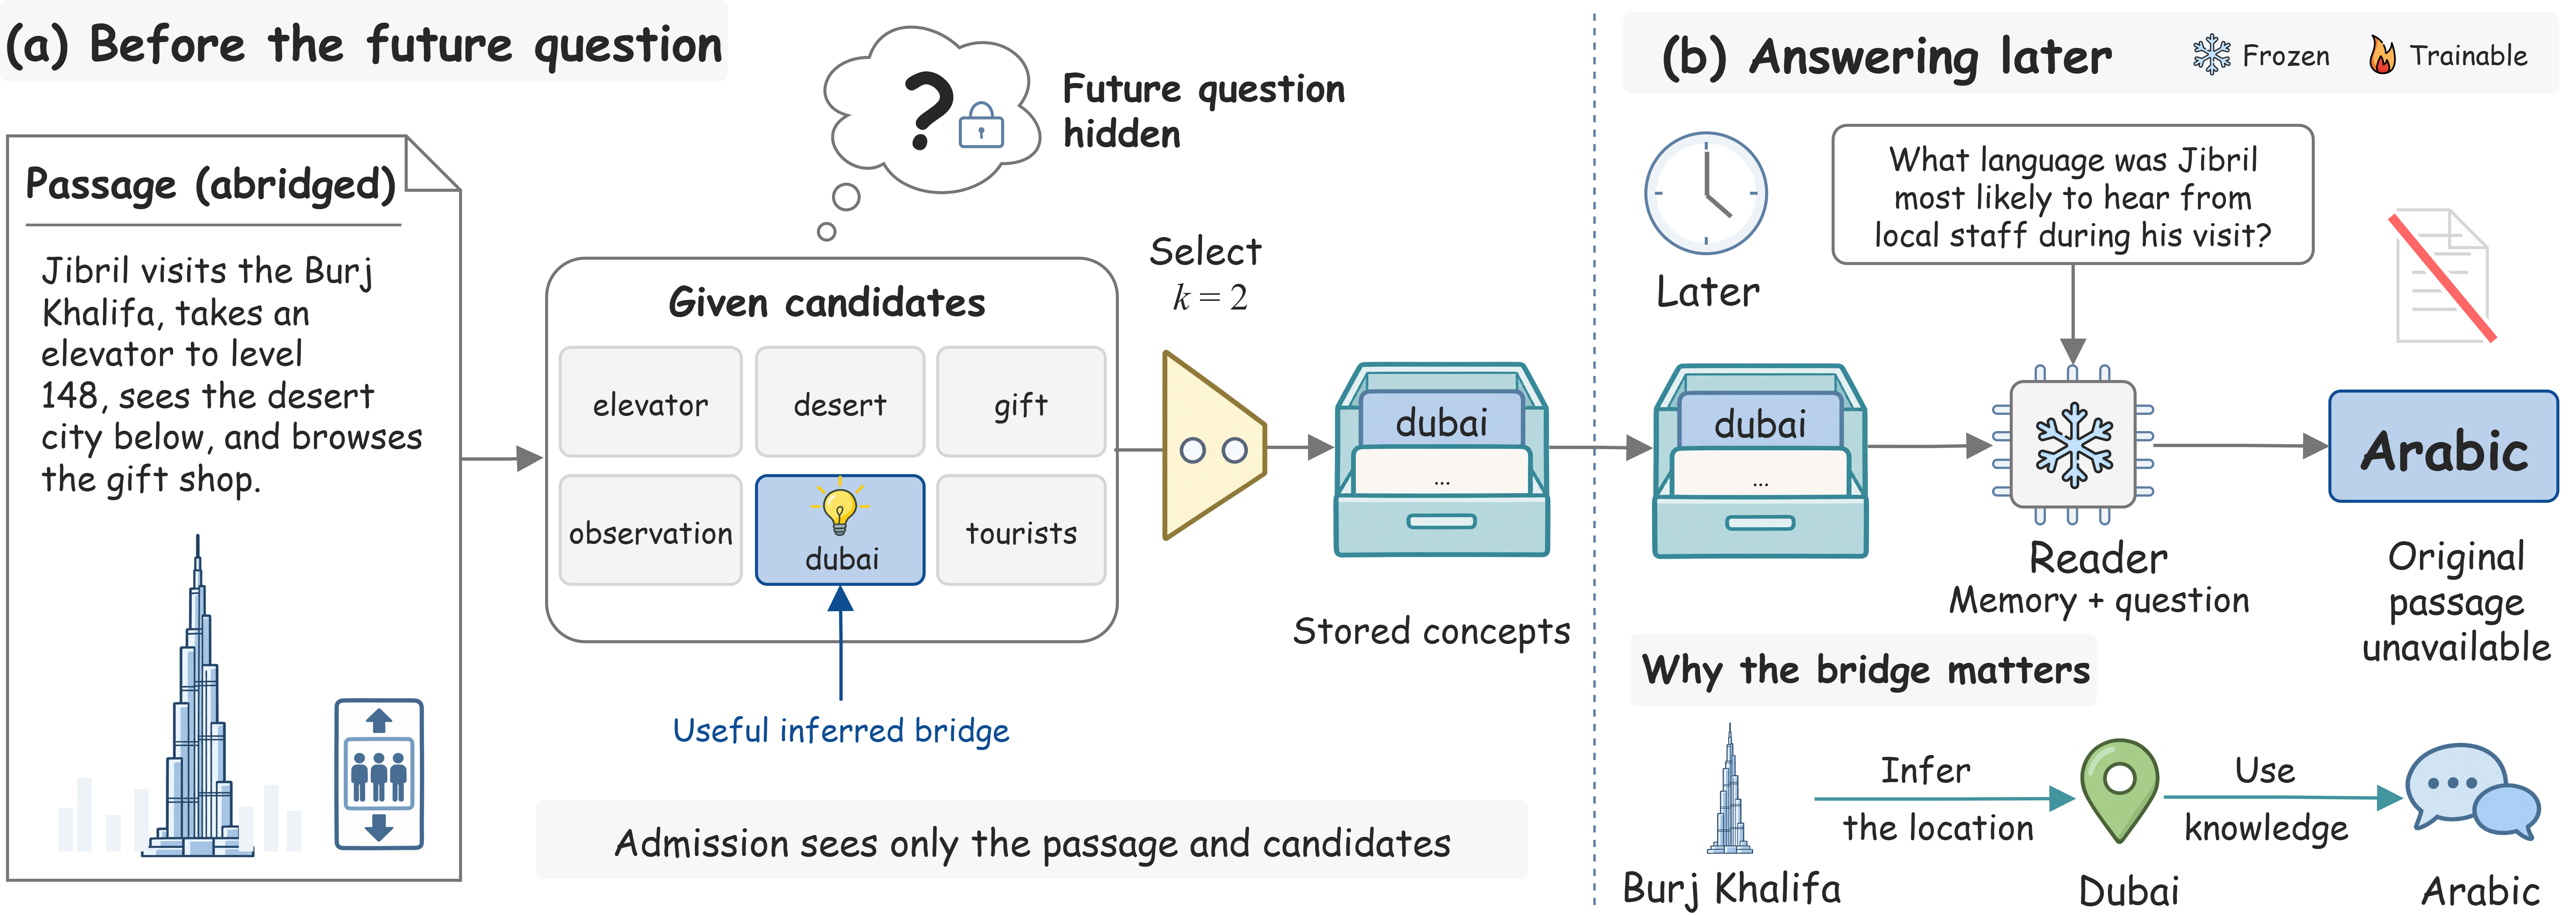
\includegraphics[width=\textwidth]{figures/fig3.png}
\caption{An abridged admission episode. (a) Before the question arrives, the policy sees only the passage and candidates, storing $k=2$ concepts. The useful concept, \emph{dubai}, is the sole unstated candidate. (b) Later, the frozen reader answers from stored concepts without the passage. Figure~\ref{fig:examples} gives the full episode.}
\label{fig:episode}
\end{figure*}

A candidate is stated if a case-insensitive stem match finds it in the passage, and unstated otherwise. Statedness AUC replaces utility labels with statedness labels.

The original pool contains the generator's candidates for 363 test-set episodes: 1,607 candidates, 4.43 per episode. In 95\% of episodes, the useful concept is the sole unstated candidate, so admitting unstated candidates first exploits this composition.

The statedness-balanced pool removes this shortcut and is the main evaluation pool. In fixed test-set order, odd positions keep the passage; even positions append ``The passage also mentions \emph{concept}.'', naming the useful concept. Episodes retain original candidates and add the first four (odd positions) or three (even positions) unstated distractors from the pool with unstated distractors. Position alone determines naming and distractor count (App.~\ref{app:pools}). The pool has 190 stated-concept and 173 unstated-concept episodes, averaging 7.93 candidates; useful concepts constitute 13.3\% of stated and 12.0\% of unstated candidates. A statedness-only rule ranks near chance: pooled AUC 0.515, within-episode AUC 0.516. Every pool preserves questions, answers and utility labels; added candidates are negative. Remaining pools and controls appear where used (\S\ref{sec:budgets}, \S\ref{sec:ablations}) and in App.~\ref{app:pools}.

Within-episode AUC averages correct useful-concept comparisons, giving ties half credit. For useful concept $b_i$, score $s$ and $n$ episodes:
\begin{equation}
\begin{split}
A_{\mathrm{episode}}&=\frac{1}{n}\sum_{i=1}^{n}\frac{\sum_{c\in C_i\setminus\{b_i\}}\phi(s(b_i),s(c))}{|C_i|-1},\\
\phi(u,v)&=\mathbf{1}\{u>v\}+\tfrac12\mathbf{1}\{u=v\}.
\end{split}
\label{eq:episodeauc}
\end{equation}
Pooled AUC compares candidates across episodes. Useful-concept retention is $B_k=\frac{1}{n}\sum_{i=1}^{n}\mathbf{1}\{b_i\in K_i\}$. Answer accuracy is the fraction of questions answered correctly by a fixed frozen reader using greedy decoding, with Qwen3 thinking disabled and a blind semantic judge. String-match agreement is 85.1\%; SDA exceeds the importance report under both graders (App.~\ref{app:judge}). Gold-concept selection ranks the useful concept first as a reference row; closed-book (question only) and full-context (whole passage) readers provide references.

SDA covers six models: Qwen3-8B, Qwen3-14B, Qwen3-32B, Qwen2.5-7B, OLMo-2-7B and Mistral-7B \citep{qwen2025,olmo2,jiang2023mistral,qwen3}; each supplies its own teacher, adapter and frozen reader. Training and validation use 175 and 45 episodes from Explicit and implied-answer constructions (App.~\ref{app:training}). Development sets select configurations; the 363-episode test set and 316-episode held-out set serve only evaluation, with budgets $k=1,2,3$.

Baselines comprise the untrained model's importance report and 1--10 importance rating, rewordings of the importance prompt, ConsistencyGate, A-MAC, Nemori and statedness rules admitting unstated candidates first (App.~\ref{app:baselines}). Trained results average three training runs; policy differences compare these means. Serving and useful-concept replacement use one reference run. Bold table entries identify SDA.
